\documentclass[compress]{beamer}
%\documentclass[noteonly]{beamer}

\usepackage[OT4]{fontenc}
\usepackage[utf8]{inputenc}
\usepackage[polish]{babel}

\usepackage{listings}

\usepackage{color}
\usepackage{xcolor}

\usetheme{Boadilla}
\usepackage{beamerthemesplit}

\usepackage{graphicx}

\xdefinecolor{nvidia}{rgb}{0.463,0.725,0.0}

\usenavigationsymbolstemplate{}
\usefonttheme{professionalfonts}

\lstset{ %
language=XML,                % choose the language of the code
basicstyle=\scriptsize,       % the size of the fonts that are used for the code
keywordstyle={\color{nvidia}\textbf},
commentstyle={\color{gray}\textit},
backgroundcolor=\color{white},  % choose the background color. You must add \usepackage{color}
showspaces=false,               % show spaces adding particular underscores
showstringspaces=false,         % underline spaces within strings
showtabs=false,                 % show tabs within strings adding particular underscores
frame=single,	                % adds a frame around the code
tabsize=4,	                % sets default tabsize to 2 spaces
captionpos=b,                   % sets the caption-position to bottom
breaklines=true,                % sets automatic line breaking
breakatwhitespace=false,        % sets if automatic breaks should only happen at whitespace
title=\lstname,                 % show the filename of files included with \lstinputlisting; also try caption instead of title
escapeinside={\%*}{*)},          % if you want to add a comment within your code
}

\title[Data reliability and integrity in federated cloud storage]{\textbf{Managing data reliability and integrity in federated cloud storage}}
\author[Krzysztof Styrc AGH]{
Krzysztof Styrc\\
\vspace{0.2cm}
\tiny
AGH University of Science and Technology, Kraków\\
\noindent
kstyrc@gmail.com\\
\vspace{0.5cm}
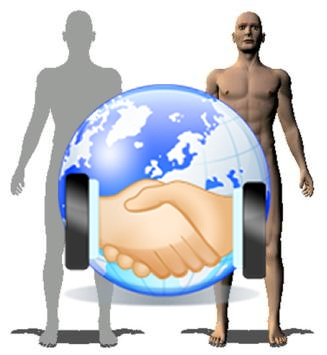
\includegraphics[height=0.2\textheight]{img/vph-share.jpg}\\
\vspace{0.5cm}
\normalsize
\hspace{5.4cm}
Supervisor: Marian Bubak, PhD\\
\hspace{4.5cm}
Advisor: Piotr Nowakowski\\
}

\date{}

\begin{document}

\frame{\titlepage}

\begin{frame}
\frametitle{\textbf{Agenda}}
	\footnotesize
	\tableofcontents
\end{frame}

\section{Background}

\subsection{Objectives}
\begin{frame}
\frametitle{Objectives}
\begin{block}{\textbf{Data in VPH-Share Cloud Platform:}}
\begin{itemize}
	\item \textbf{sensitive} data on one or more cloud storage nodes (S3, Swift, \ldots),
	\item data has to be \textbf{available} and \textbf{valid}.
\end{itemize}
\end{block}
\begin{exampleblock}{\textbf{The aims of this work:}}
	\begin{enumerate}
		\item \textbf{efficient} data validation mechanism in federated cloud storage,
		\item implementation under various practical \textbf{limitations}.
	\end{enumerate}
\end{exampleblock}
\begin{block}{\textbf{Essentials aspects of this work:}}
\begin{itemize}
	\item design and implementation of DRI REST WS enabling data validation,
	\item integration with the VPH-Share Cloud Platform environment,
	\item design of a bandwidth-efficient validation algorithm
\end{itemize}
\end{block}
\end{frame}

\subsection{Motivation}
\begin{frame}
\frametitle{\textbf{Data integrity in cloud storage}}
\begin{block}{\textbf{Why data validation in cloud storage?}}
SLA guarantes $99.9\%$, if not met -- credit return:\\
\textit{-- http://aws.amazon.com/s3-sla/\\
-- http://www.rackspace.com/cloud/legal/sla/\\
-- https://developers.google.com/appengine/sla\\
}
Moreover, in replicated environment one can use other cloud provider while primary is unavailable or contains corrupted data.
\end{block}
\begin{exampleblock}{\textbf{Recent problems with the \textit{cloud} services:}}
\begin{itemize}
	\item Gmail: erased emails, blocked accounts,
	\item Amazon S3: serving corrupted data, unavailable data,
	\item GoogleDocs: unauthorized data access,
\end{itemize}
\end{exampleblock}
\end{frame}

\section{Design}

\subsection{VPH-Share}
\begin{frame}
\frametitle{\textbf{VPH-Share environment}}
\begin{itemize}
	\item \textbf{Atmosphere Internal Registry} (AIR) -- metadata database of datasets, files, storage nodes, configuration, policy,
	\item data structure: \textit{dataset = set of files}
	\begin{figure}
		\centering
		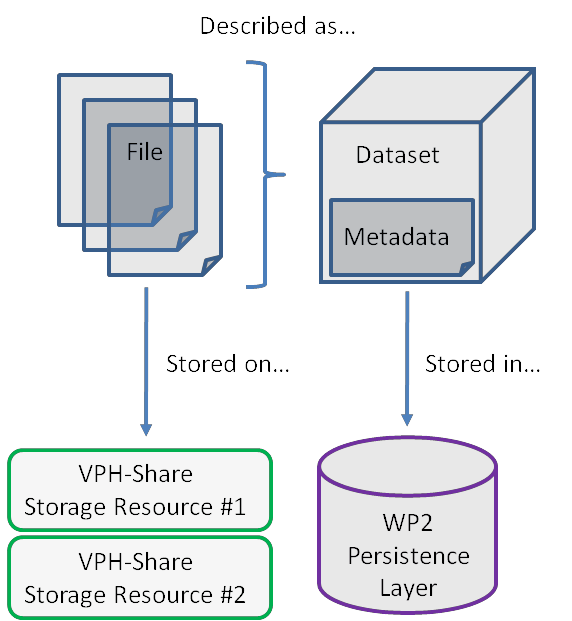
\includegraphics[scale=0.15]{img/managed-dataset.png}
		\hspace{1cm}
		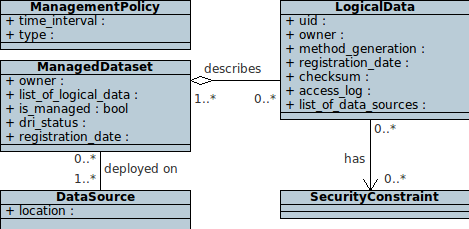
\includegraphics[scale=0.4]{img/data_model.png}
	\end{figure}
\end{itemize}

\begin{exampleblock}{}
	\begin{columns}
		\begin{column}{0.6\textwidth}
			\textbf{Storage nodes} -- direct access to cloud storage nodes rather than LOBCDER layer (S3, Swift, \ldots).
		\end{column}
		\begin{column}{0.3\textwidth}
			\centering
			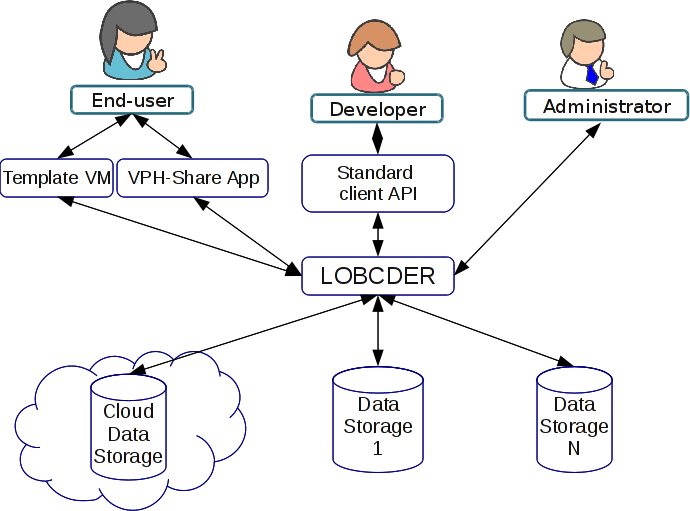
\includegraphics[scale=0.12]{img/lobcder.png}
		\end{column}
	\end{columns}
\end{exampleblock}
\end{frame}

\begin{frame}
\begin{figure}
	\centering
	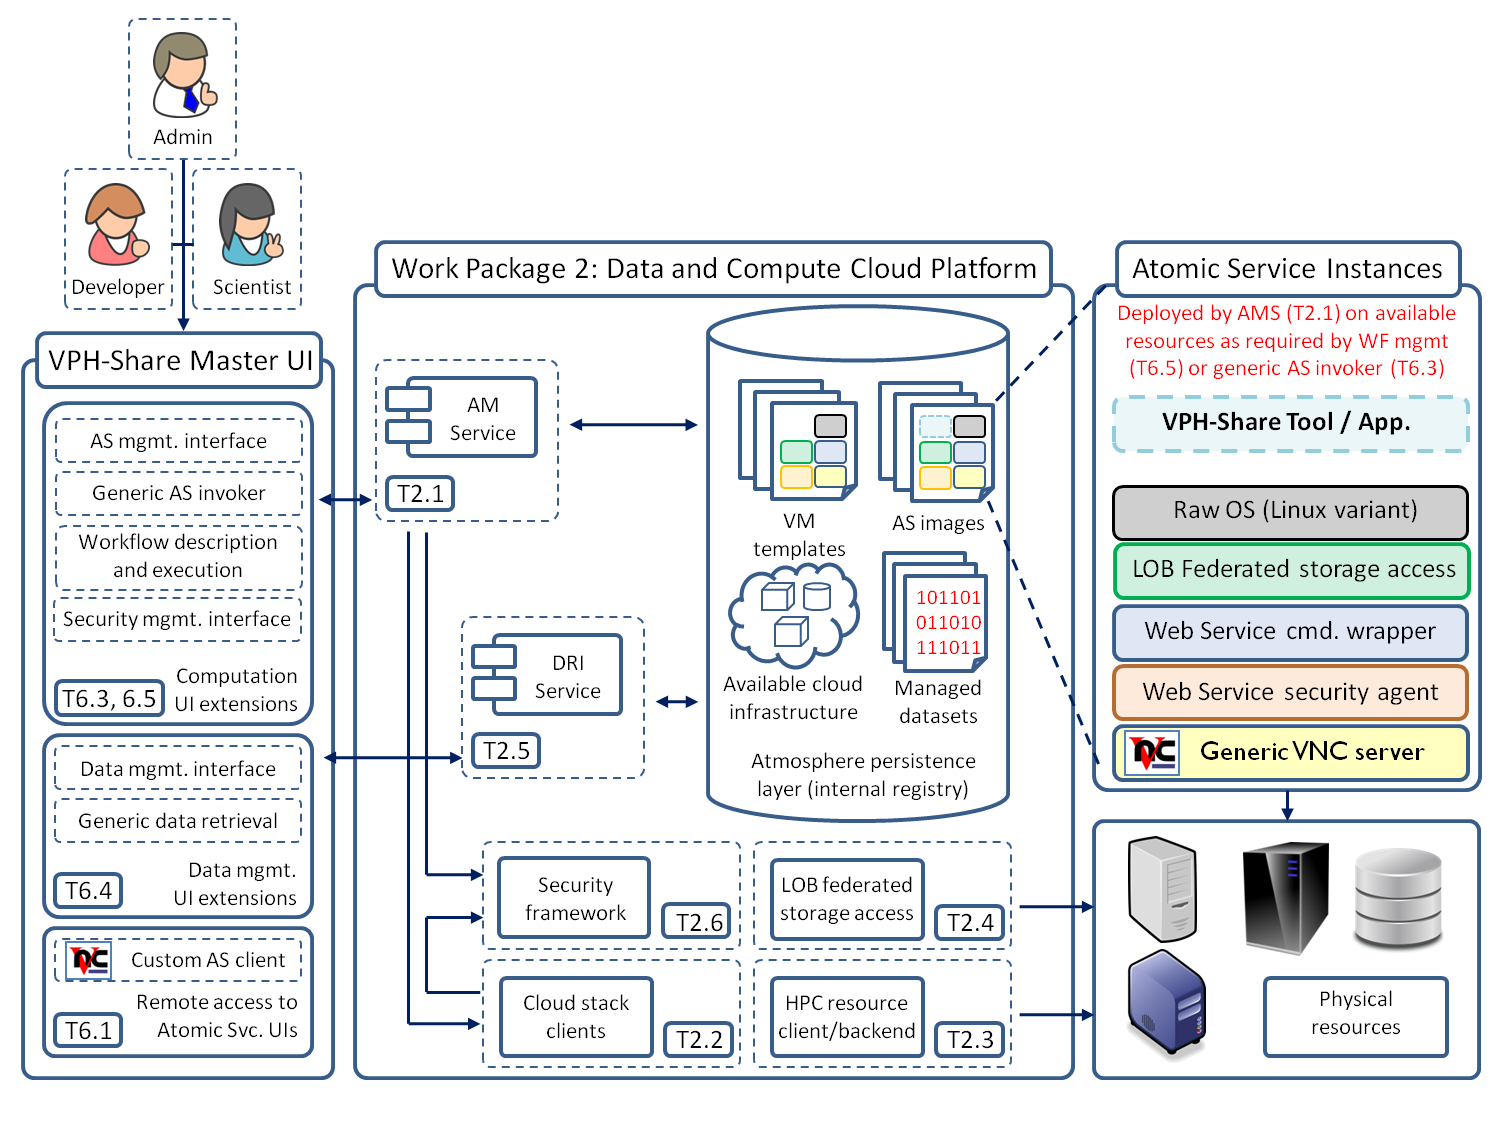
\includegraphics[height=0.7\textheight]{img/cloud-platform.png}
\end{figure}
\begin{columns}
	\begin{column}{0.48\textwidth}
		\begin{block}{\small\textbf{Functional requirements:}}
		\tiny
			\begin{itemize}
				\item periodic and on-request validation,
				\item data replication,
				\item user notification about integrity errors.
			\end{itemize}
		\end{block}
	\end{column}
	\begin{column}{0.48\textwidth}
		\begin{block}{\small\textbf{Nonfunctional requirements:}}
		\tiny
			\begin{itemize}
				\item \textbf{bandwidth-efficient} validation mechanism,
				\item scalablility,
				\item configurability.
			\end{itemize}
		\end{block}
	\end{column}
\end{columns}
\end{frame}

\subsection{Architecture}
\begin{frame}
\frametitle{\textbf{DRI architecture}}
\begin{figure}
	\centering
	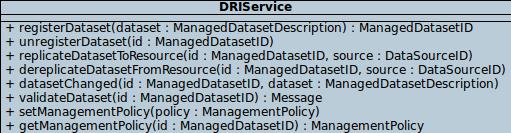
\includegraphics[height=0.3\textheight]{img/dri_interface.png}\\
	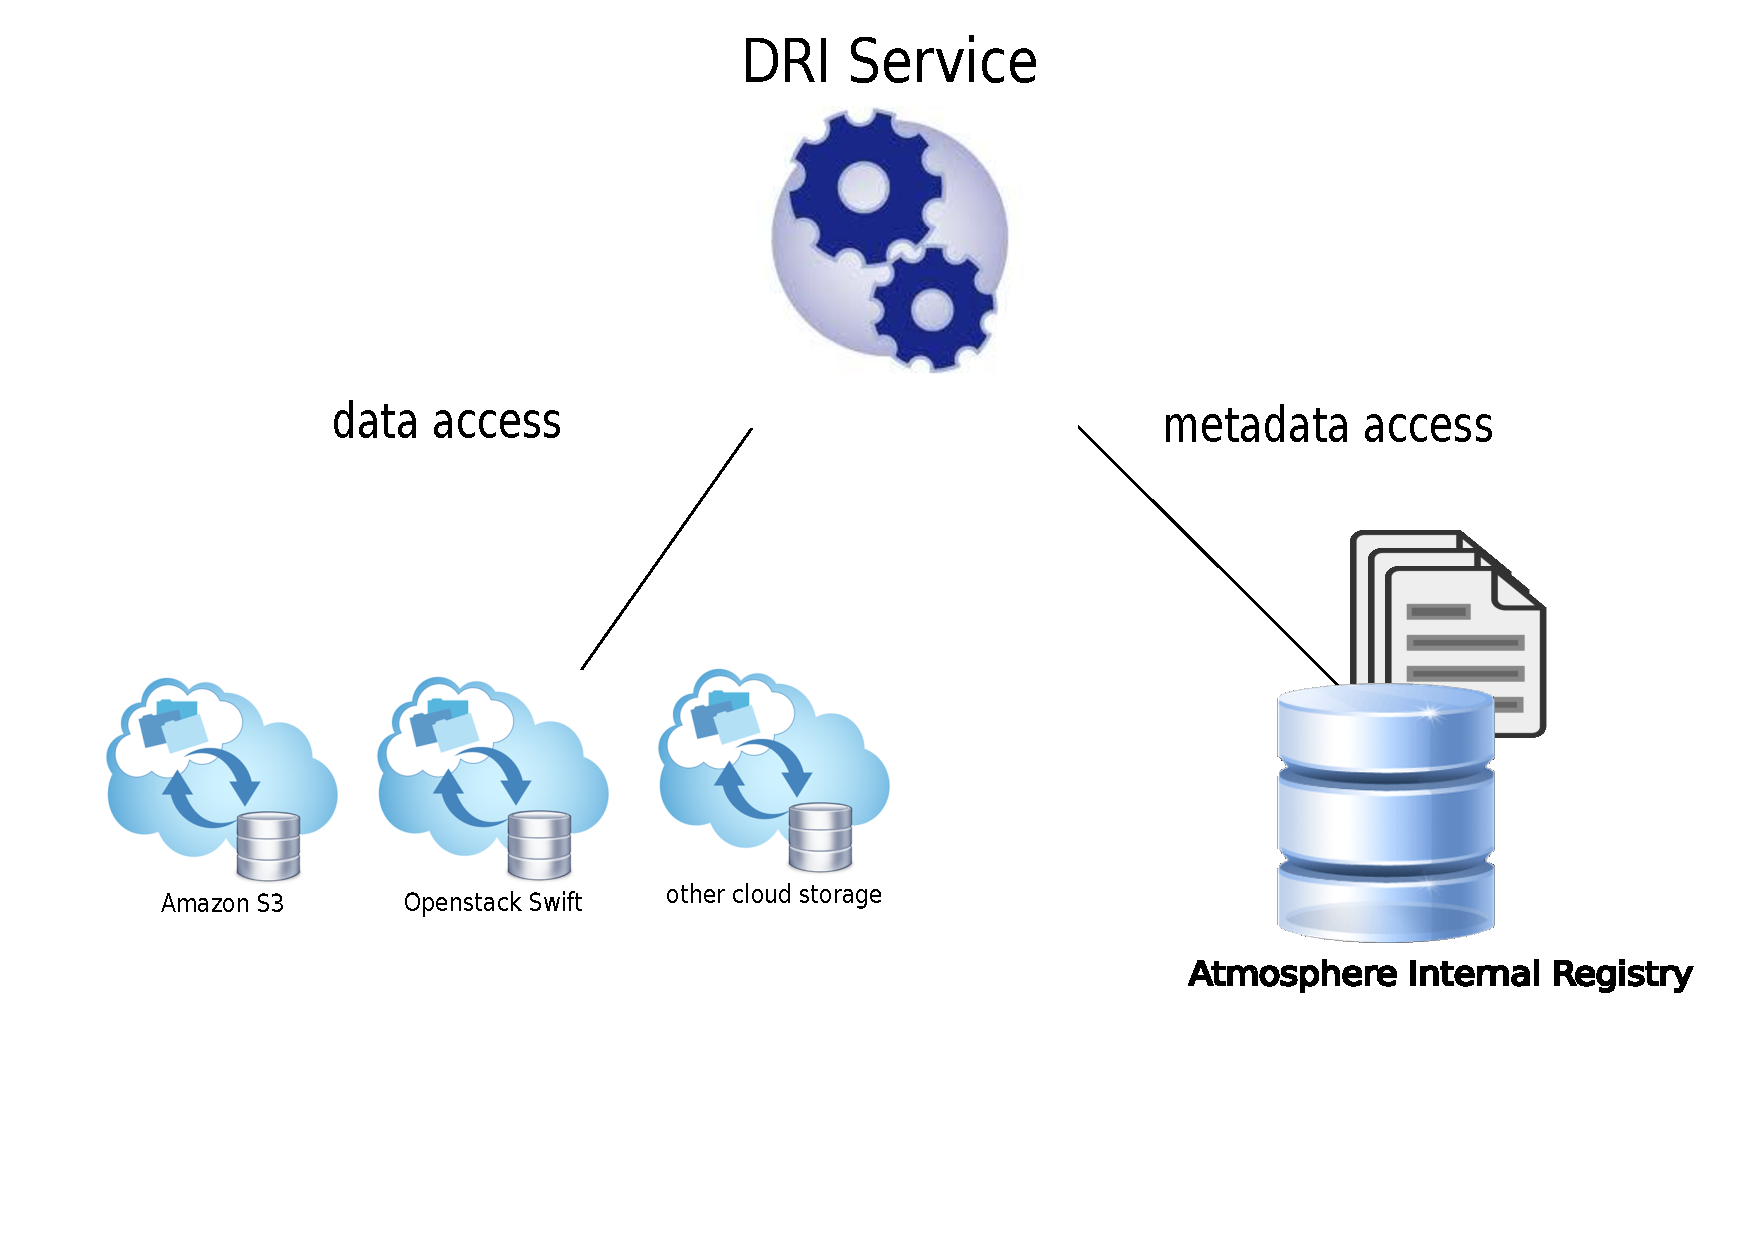
\includegraphics[height=0.7\textheight]{img/schemat.pdf}
\end{figure}
\end{frame}

\begin{frame}
\begin{figure}
	\centering
	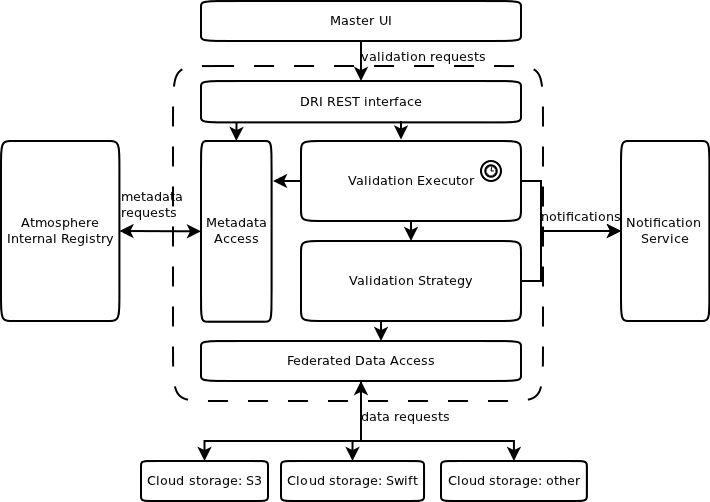
\includegraphics[height=0.8\textheight]{img/design.png}
\end{figure}
\end{frame}

\section{Validation}

\subsection{Cloud storage}
\begin{frame}
\frametitle{\textbf{Cloud storage characteristics}}
\begin{itemize}
	\item hierarchical structure: \textit{account / container / object},
	\item typical operations: \textit{list, get, put, delete, update, \ldots},
	\item REST API goes toward CDMI/OCCI standards:\\
		\tiny
		\textit{-- http://docs.amazonwebservices.com/AmazonS3/latest/API/\\
			-- http://docs.openstack.org/api/openstack-object-storage/1.0/content/\\
			-- http://docs.rackspace.com/files/api/v1/cf-devguide/content/index.html\\
		}
		\normalsize
	\item SLA quality, best quality--price ratio, scalability, \ldots,
\end{itemize}
\begin{block}{\textbf{No support for HTTP Multi-Range requests:}}
\begin{itemize}
	\item new request for every chunk,
	\item flooding the cloud storage,
	\item really bad performance $\rightarrow$ RTT for every chunk.
\end{itemize}
\end{block}
\end{frame}

\subsection{Algorithm}
\begin{frame}
\frametitle{\textbf{Validation algorithm pseudocode}}
\begin{figure}
	\centering
	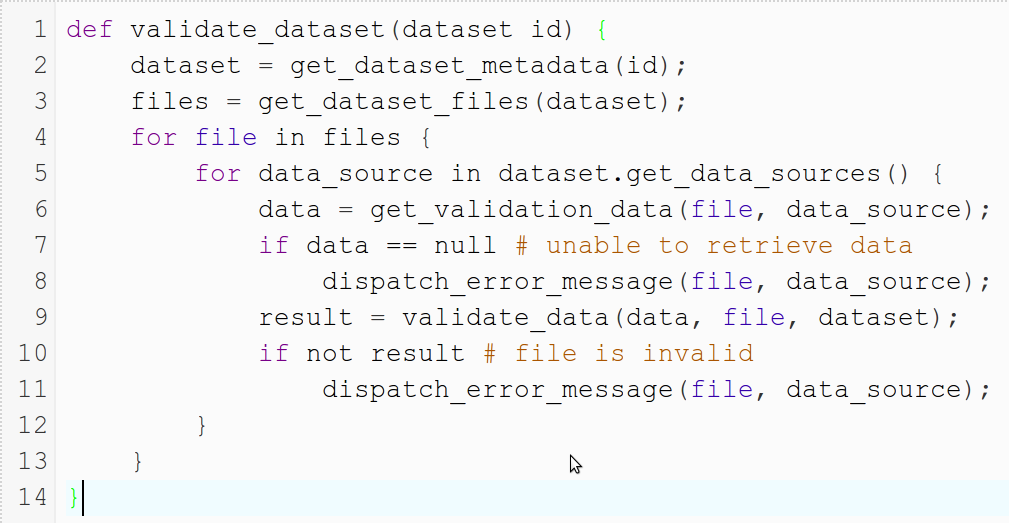
\includegraphics[width=\textwidth]{img/algorithm.png}
\end{figure}
\end{frame}

\begin{frame}
\frametitle{\textbf{Validation algorithm sequence diagram}}
\begin{figure}
	\centering
	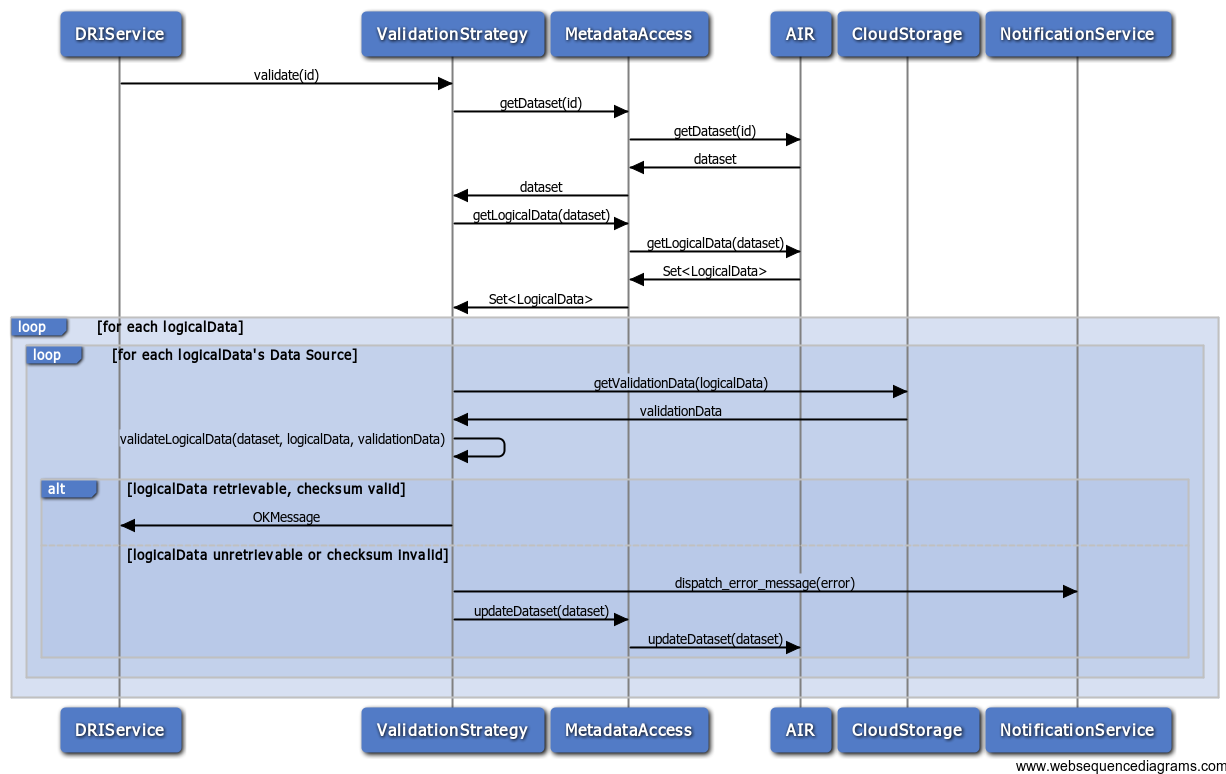
\includegraphics[width=\textwidth]{img/algorithm2.png}
\end{figure}
\end{frame}

\subsection{Technologies}
\begin{frame}
\frametitle{\textbf{Implementation technologies}}
\begin{itemize}
	\item \textbf{Jersey API} -- JAX-RS reference implementation, REST communication
	\item \textbf{JClouds} -- very good cloud operability library,
	\item \textbf{Quartz} -- tasks execution and scheduling library,
	\item \textbf{Guice} -- dependency injection and modularity library,
	\item \textbf{Maven} -- build + dependencies tool,
	\item \textbf{Apache Tomcat} -- server. 
\end{itemize}
\end{frame}

\subsection{Efficiency}
\begin{frame}
\frametitle{\textbf{Validation efficiency}}
\begin{block}{}
Significant size of data stored in federated cloud storage makes whole-file checksum-based validation completely inefficient. 
Additionally, occupying substantial portion of network bandwidth is highly undesirable.\\
\textbf{For example:}\\
typical dataset $\approx$ 10 GB $\rightarrow$ goal: reduce to $\approx 10\%$
\end{block}
\begin{exampleblock}{}
\textbf{Can we do better?}\\
Generally yes, but lots of practical limitations:
\begin{itemize}
	\item cloud storage limitations,
	\item files cannot be modified in VPH-Share.
\end{itemize}
\textbf{Promising approaches:}\\
\begin{enumerate}
	\item Proofs of Retrievability (PoR),
	\item Data integrity proofs (DIP).
\end{enumerate}
\end{exampleblock}
\end{frame}

\section{Approaches}

\subsection{Classic}
\begin{frame}
\frametitle{\textbf{Classical integrity mechanisms}}
\begin{itemize}
	\footnotesize
	\item \textbf{Hash functions} -- for detecting data corruption (MD5, SHA1, \ldots),
	\item \textbf{Error Correcting Codes (ECC)} -- for correcting small parts of data,
	\item \textbf{Message Authentication Codes (MAC)} -- hash + auth\_key for secure authentication.
\end{itemize}
\begin{columns}
	\begin{column}{0.5\textwidth}
	\begin{block}{}
		Validation mechanism steps:
		\begin{enumerate}
			\item setup: compute and store,
			\item validate: compute + compare.
		\end{enumerate}
	\end{block}
	\end{column}
	\begin{column}{0.5\textwidth}
		\begin{figure}
			\centering
			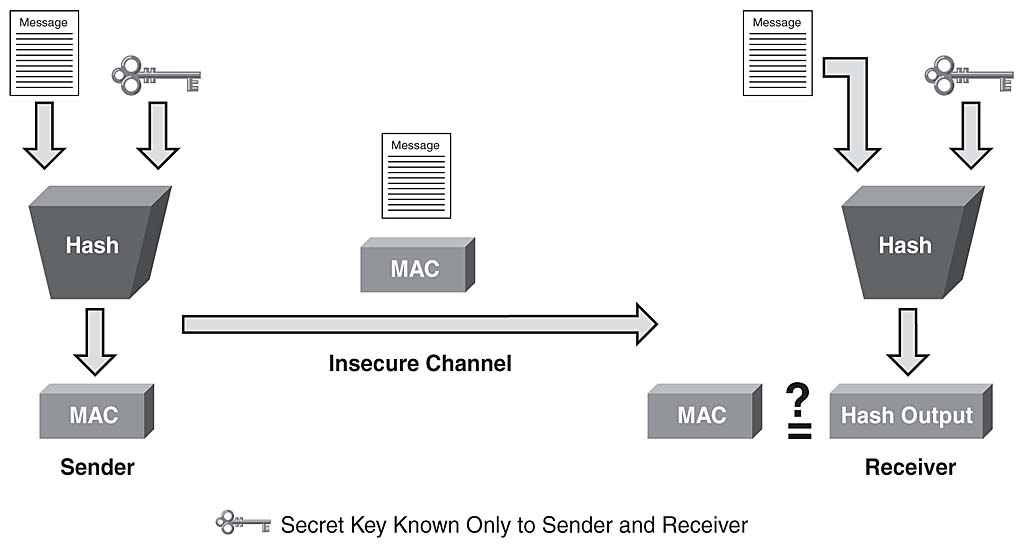
\includegraphics[height=0.3\textheight]{img/hmac.jpg}
		\end{figure}
	\end{column}
\end{columns}
\end{frame}

\subsection{PoR}
\begin{frame}
\frametitle{\textbf{Proofs of Retrievability scheme}}
\begin{columns}
	\begin{column}{0.5\textwidth}
		\small
		\textbf{Setup:}
		\begin{enumerate}
			\item divide into chunks,
			\item compute ECC + MAC,
			\item ${F^{*} \over F} \approx 102-115\%$.
		\end{enumerate}
		\textbf{Validation:}
		\begin{enumerate}
			\item challenge--response rounds:
			\item more rounds $\rightarrow$ higher probability,
			\item more rounds $\rightarrow$ higher bandwidth.
		\end{enumerate}
		\textbf{Problems:}
		\begin{enumerate}
			\item we cannot modify stored file,
			\item data is served by LOBCDER, ECC useless.
		\end{enumerate}
	\end{column}
	\begin{column}{0.5\textwidth}
		\begin{figure}
			\centering
			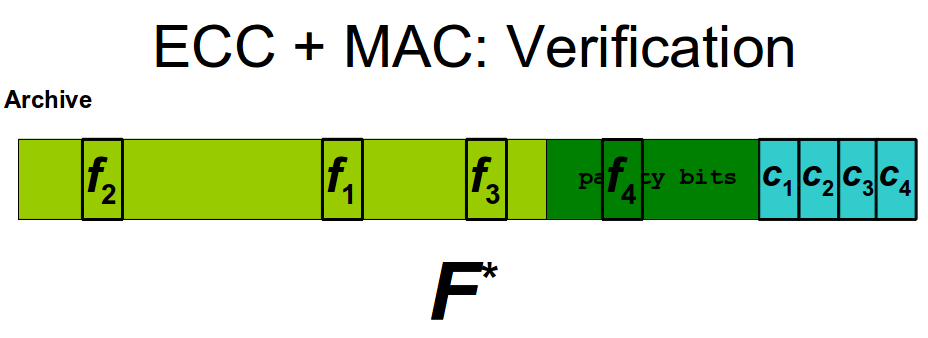
\includegraphics[width=\textwidth]{img/modified_file.png}\\
			\vspace{1cm}
			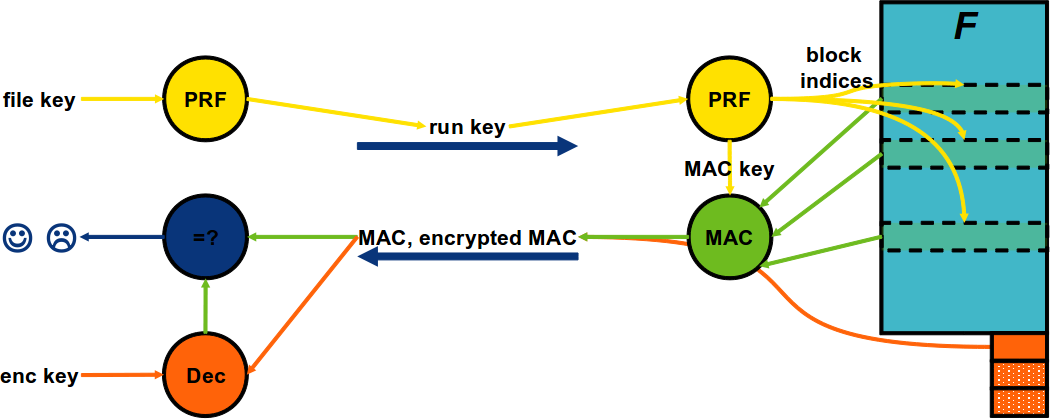
\includegraphics[width=\textwidth]{img/por-diagram.png}
		\end{figure}
	\end{column}
\end{columns}
\end{frame}

\subsection{DIP}
\begin{frame}
\frametitle{\textbf{Data integrity proofs scheme}}
\begin{columns}
	\begin{column}{0.5\textwidth}
		\small
		\textbf{Setup:}
		\begin{enumerate}
			\item divide into $k$ chunks,
			\item pick $m$ bits in every chunk,
			\item compute MAC and store.
		\end{enumerate}
		\textbf{Validation:}
		\begin{enumerate}
			\item compute as in setup,
			\item compare with original MAC.
		\end{enumerate}
		\textbf{Problems:}
		\begin{enumerate}
			\item cannot query cloud storage bit by bit,
			\item cannot append to stored file.
		\end{enumerate}
	\end{column}
	\begin{column}{0.5\textwidth}
		\begin{figure}
			\centering
			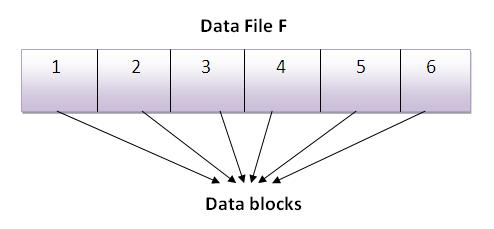
\includegraphics[width=0.8\textwidth]{img/dip1.png}\\
			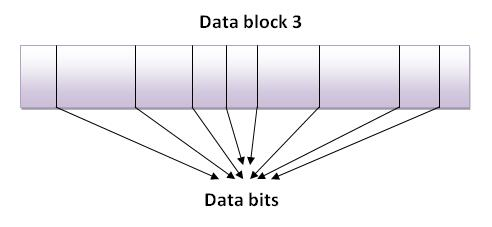
\includegraphics[width=0.8\textwidth]{img/dip2.png}\\
			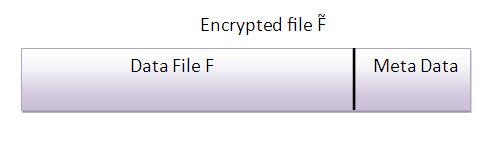
\includegraphics[width=0.8\textwidth]{img/dip3.png}
		\end{figure}
	\end{column}
\end{columns}
\end{frame}

\subsection{Solution}
\begin{frame}
\frametitle{\textbf{Our solution -- mixed PoR + DIP}}
\begin{columns}
	\begin{column}{0.5\textwidth}
		\small
		\textbf{Setup:}
		\begin{enumerate}
			\item divide into chunks of size $S$,
			\item compute MAC of every single chunk and store.
		\end{enumerate}
		\textbf{Validation:}
		\begin{enumerate}
			\item pick sequence of $k$ random indexes (Mersenne-Twister),
			\item get $k$ chunks data,
			\item compute and verify with originals.
		\end{enumerate}
		\textbf{Solution features:}
		\begin{itemize}
			\item configurable accuracy--overhead ratio,
			\item practical feasibility.
		\end{itemize}
	\end{column}
	\begin{column}{0.5\textwidth}
		\begin{figure}
			\centering
			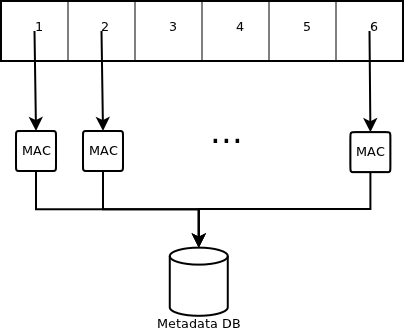
\includegraphics[width=0.6\textwidth]{img/solution-setup.png}\\
			\vspace{0.5cm}
			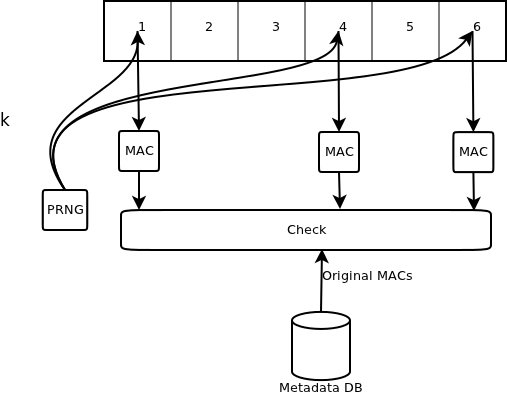
\includegraphics[width=0.7\textwidth]{img/solution-validation.png}
		\end{figure}
	\end{column}
\end{columns}
\end{frame}



\section{Conclusions}
\begin{frame}
\begin{block}{\textbf{Work status:}}
\begin{itemize}
	\item working periodic and on-request validation,
	\item integrity errors notifications page,
	\item task scheduling + configurability,
	\item \textbf{testing the implementation of our solution},
	\item \textbf{thesis writing start}.
\end{itemize}
\end{block}
\begin{exampleblock}{\textbf{Conclusions:}}
	\begin{itemize}
		\item cloud storages have their usability limitations,
		\item remote data validation -- not a trivial task,
		\item efficient validation only with high probability.
	\end{itemize}
\end{exampleblock}
\begin{block}{\textbf{Future work:}}
\begin{itemize}
	\item integrate LOBCDER and DRI tools,
	\item watch future versions of CDMI/OCCI standards for significant impovements. 
\end{itemize}
\end{block}
\end{frame}

\end{document}
